\chapter{Aims and hypothesis}

\noindent   % First paragraph has no indentation.
First paragraph in current heading. First paragraph in current heading.
First paragraph in current heading. First paragraph in current heading.
First paragraph in current heading. First paragraph in current heading.
First paragraph in current heading. First paragraph in current heading.
First paragraph in current heading.

Next paragraph in current heading. Next paragraph in current heading.
Next paragraph in current heading. Next paragraph in current heading.
Next paragraph in current heading. Next paragraph in current heading.
Next paragraph in current heading. Next paragraph in current heading.
Next paragraph in current heading.

\section{A section}

\noindent   % First paragraph has no indentation.
First paragraph in current heading. First paragraph in current heading.
First paragraph in current heading. First paragraph in current heading.
First paragraph in current heading. First paragraph in current heading.
First paragraph in current heading. First paragraph in current heading.
First paragraph in current heading.

Next paragraph in current heading. Next paragraph in current heading.
Next paragraph in current heading. Next paragraph in current heading.
Next paragraph in current heading. Next paragraph in current heading.
Next paragraph in current heading. Next paragraph in current heading.
Next paragraph in current heading.

Next paragraph in current heading. Next paragraph in current heading.
Next paragraph in current heading. Next paragraph in current heading.
Next paragraph in current heading. Next paragraph in current heading.
Next paragraph in current heading. Next paragraph in current heading.
Next paragraph in current heading.

Next paragraph in current heading. Next paragraph in current heading.
Next paragraph in current heading. Next paragraph in current heading.
Next paragraph in current heading. Next paragraph in current heading.
Next paragraph in current heading. Next paragraph in current heading.
Next paragraph in current heading.

% Example: Figure composed of three subfigures
\begin{figure}[h!]
\centering
\subfigure[]{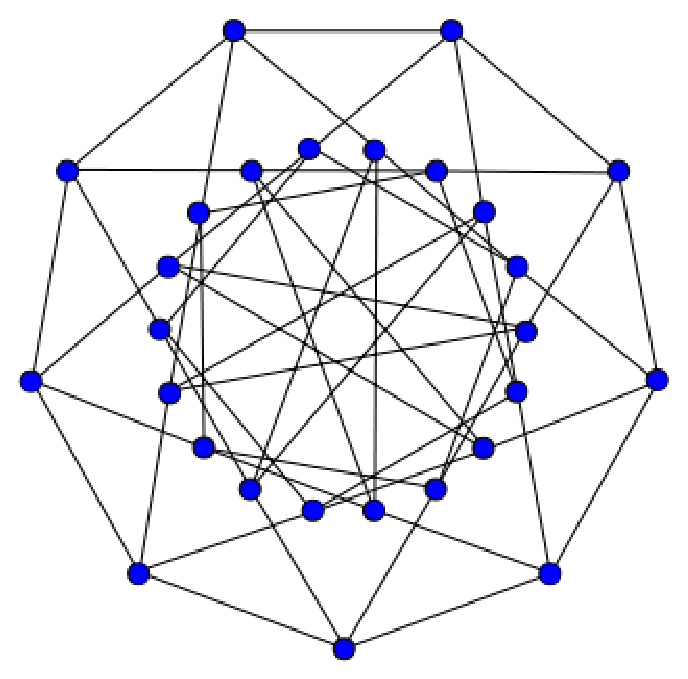
\includegraphics[width=5.1cm]{sample-3a.eps}}
\hspace{4mm}
\subfigure[]{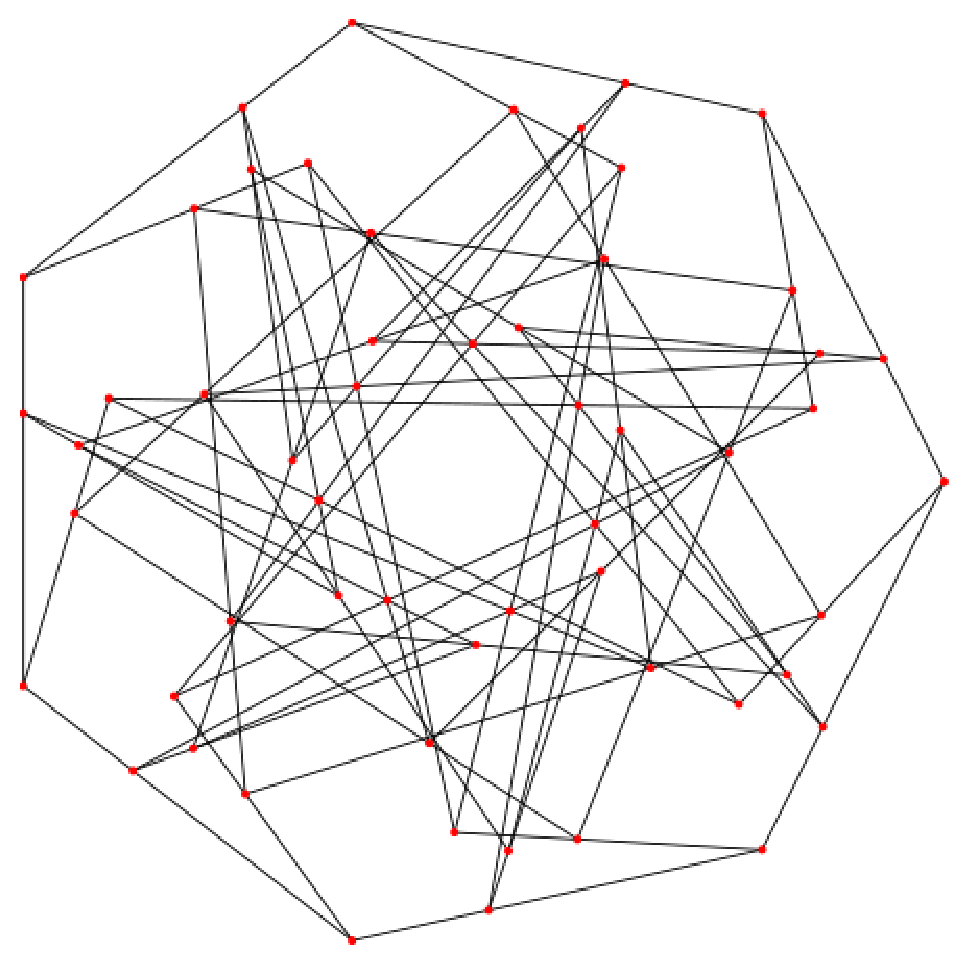
\includegraphics[width=5cm]{sample-3c.eps}}
\hspace{4mm}
\subfigure[]{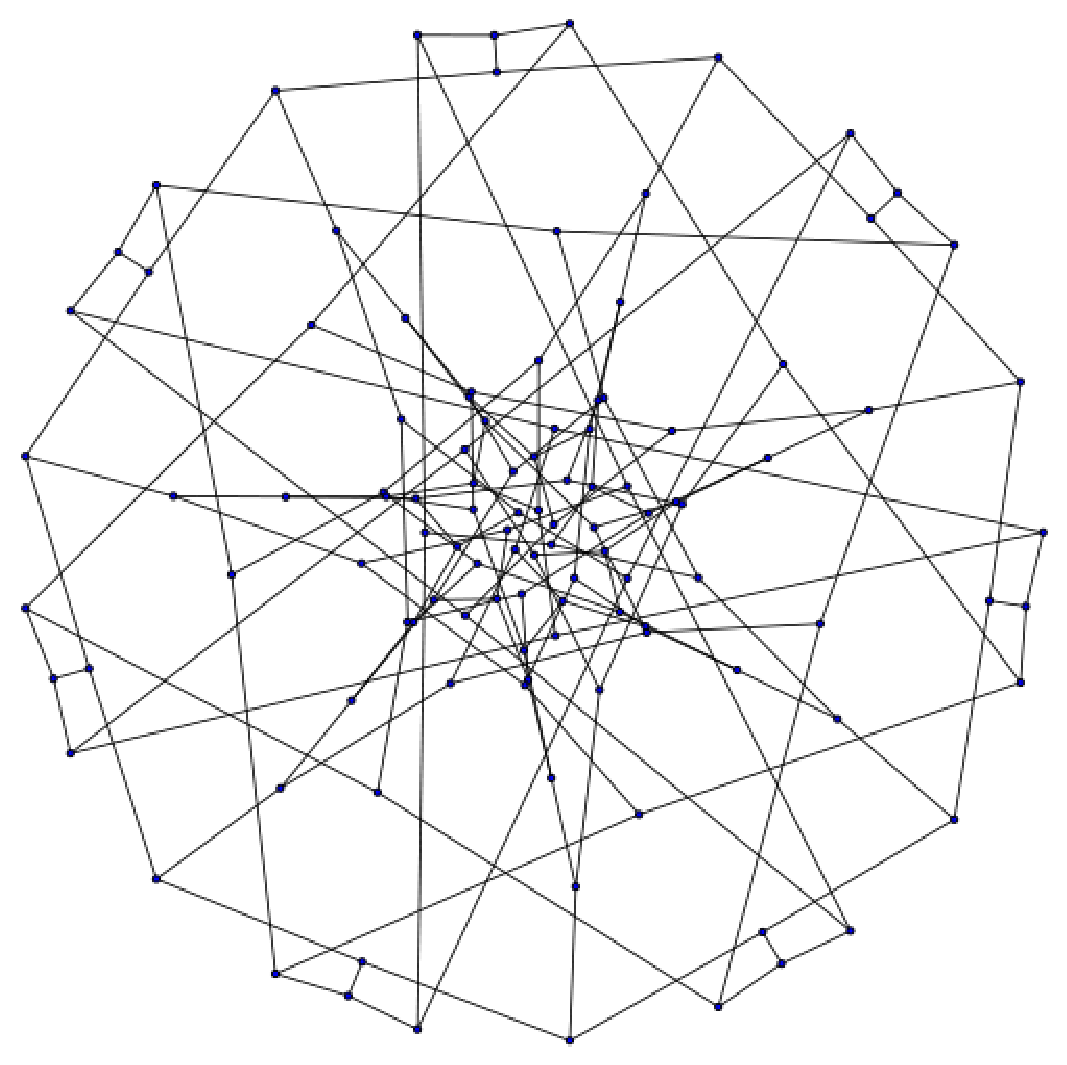
\includegraphics[width=5cm]{sample-3b.eps}}
\caption[Title.]{\textit{Title.} Caption of this figure. Caption of this figure. Caption of this figure.
Caption of this figure. Caption of this figure. Caption of this figure. Caption of this figure. Caption of this figure.}
\label{sts-resolution}
\end{figure}

Next paragraph in current heading. Next paragraph in current heading.
Next paragraph in current heading. Next paragraph in current heading.
Next paragraph in current heading. Next paragraph in current heading.
Next paragraph in current heading. Next paragraph in current heading.
Next paragraph in current heading.

    \subsection{A subsection}

\noindent   % First paragraph has no indentation.
First paragraph in current heading. First paragraph in current heading.
First paragraph in current heading. First paragraph in current heading.
First paragraph in current heading. First paragraph in current heading.
First paragraph in current heading. First paragraph in current heading.
First paragraph in current heading.

Next paragraph in current heading. Next paragraph in current heading.
Next paragraph in current heading. Next paragraph in current heading.
Next paragraph in current heading. Next paragraph in current heading.
Next paragraph in current heading. Next paragraph in current heading.
Next paragraph in current heading.

Next paragraph in current heading. Next paragraph in current heading.
Next paragraph in current heading. Next paragraph in current heading.
Next paragraph in current heading. Next paragraph in current heading.
Next paragraph in current heading. Next paragraph in current heading.
Next paragraph in current heading.


        \subsubsection{A subsubsection}

\noindent   % First paragraph has no indentation.
First paragraph in current heading. First paragraph in current heading.
First paragraph in current heading. First paragraph in current heading.
First paragraph in current heading. First paragraph in current heading.
First paragraph in current heading. First paragraph in current heading.
First paragraph in current heading.

Next paragraph in current heading. Next paragraph in current heading.
Next paragraph in current heading. Next paragraph in current heading.
Next paragraph in current heading. Next paragraph in current heading.
Next paragraph in current heading. Next paragraph in current heading.
Next paragraph in current heading.



